\chapter{Derivation of Parasite Clearance Times}
\section{Estimating the primary endpoint}
The endpoint of primary importance is PC90, the time to achieve a reduction of the parasitaemia by 90\% of baseline level. The baseline level is the pre-dose parasite count. We have data for parasite counts taken at specific times and therefore will have a measurement of the parasite count at a time when the count was above 90\% of the baseline, followed by one where it where it is below 90\% and hence we need to find an appropriate interpolation to determine a time at which the parasite count was 90\%.

As a first attempt at deriving estimates of PC90 from the data, simple linear polynomial fits to the logarithm of the parasite count with time from first dose are investigated. This is followed by non-linear logistic regression as has been used by others\cite{wootton}. We also look at simple linear or or log-linear interpolation which has also been used for data of this kind\cite{carmello}.
\subsection{Using a transformation of the count}
In the previous chapter it was noted that a logarithmic transformation was appropriate to remove the skew of the parasite count distribution. Figure \ref{raw901M} shows the untransformed parasite count for centre 1 males with a horizontal line indicating the PC90 level and Figure \ref{log901M} shows the log-transformed parasite count.

We can see that the logarithmic transformation reduces the significance of large fluctuations in the parasite count soon after first dose and brings the region around the PC90 level into greater prominence. Consequently, interpolated estimates of PC90 in these log-linear co-ordinates will be more accurate and any regression will be more influenced by data close to the region of interest.  
\begin{figure}[p]
\begin{center}
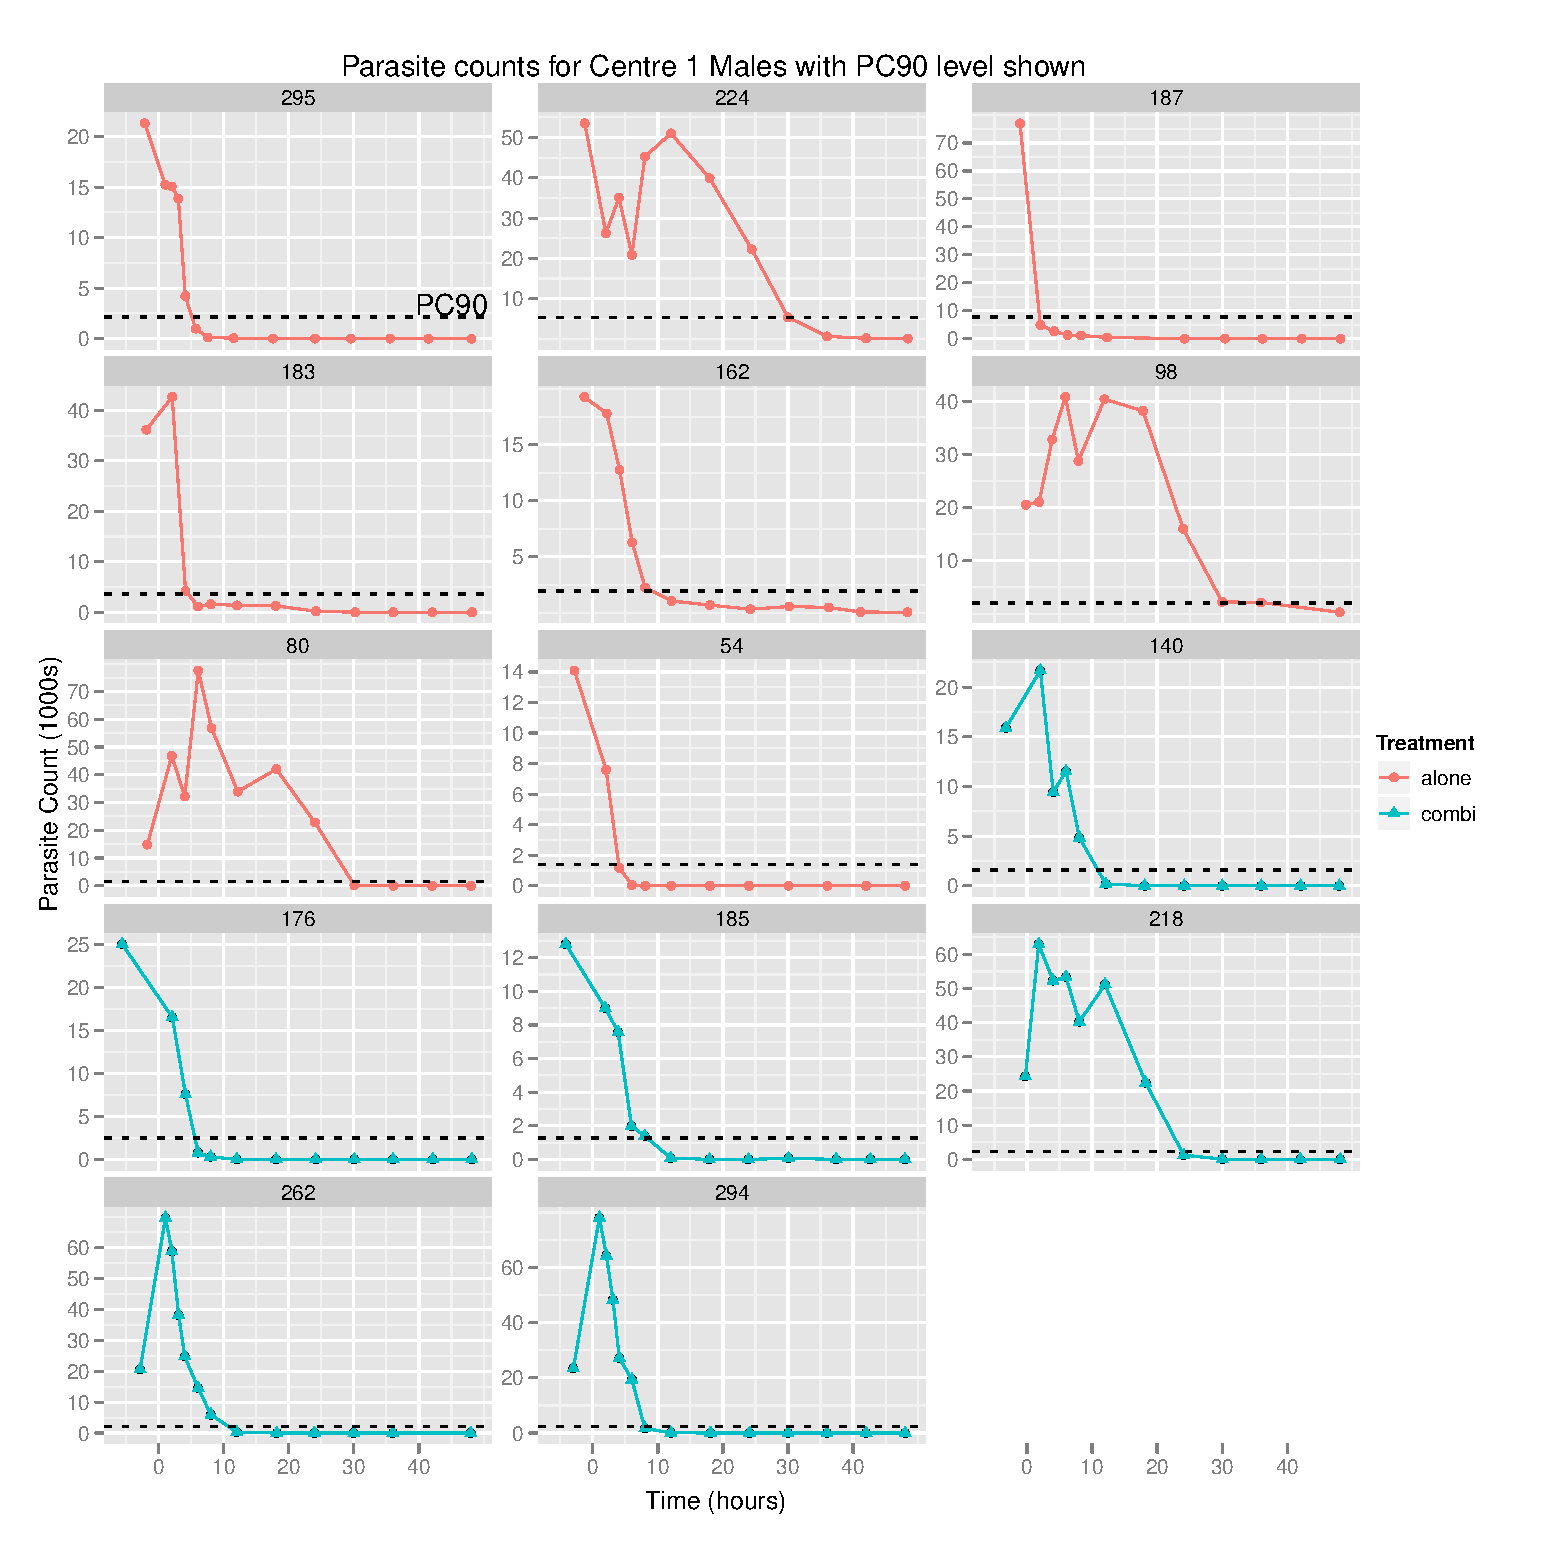
\includegraphics[width=6.1in]{raw901M.eps}
\caption{Untransformed parasite counts with PC90 level shown}
\label{raw901M}
\end{center}
\end{figure}
\begin{figure}[p]
\begin{center}
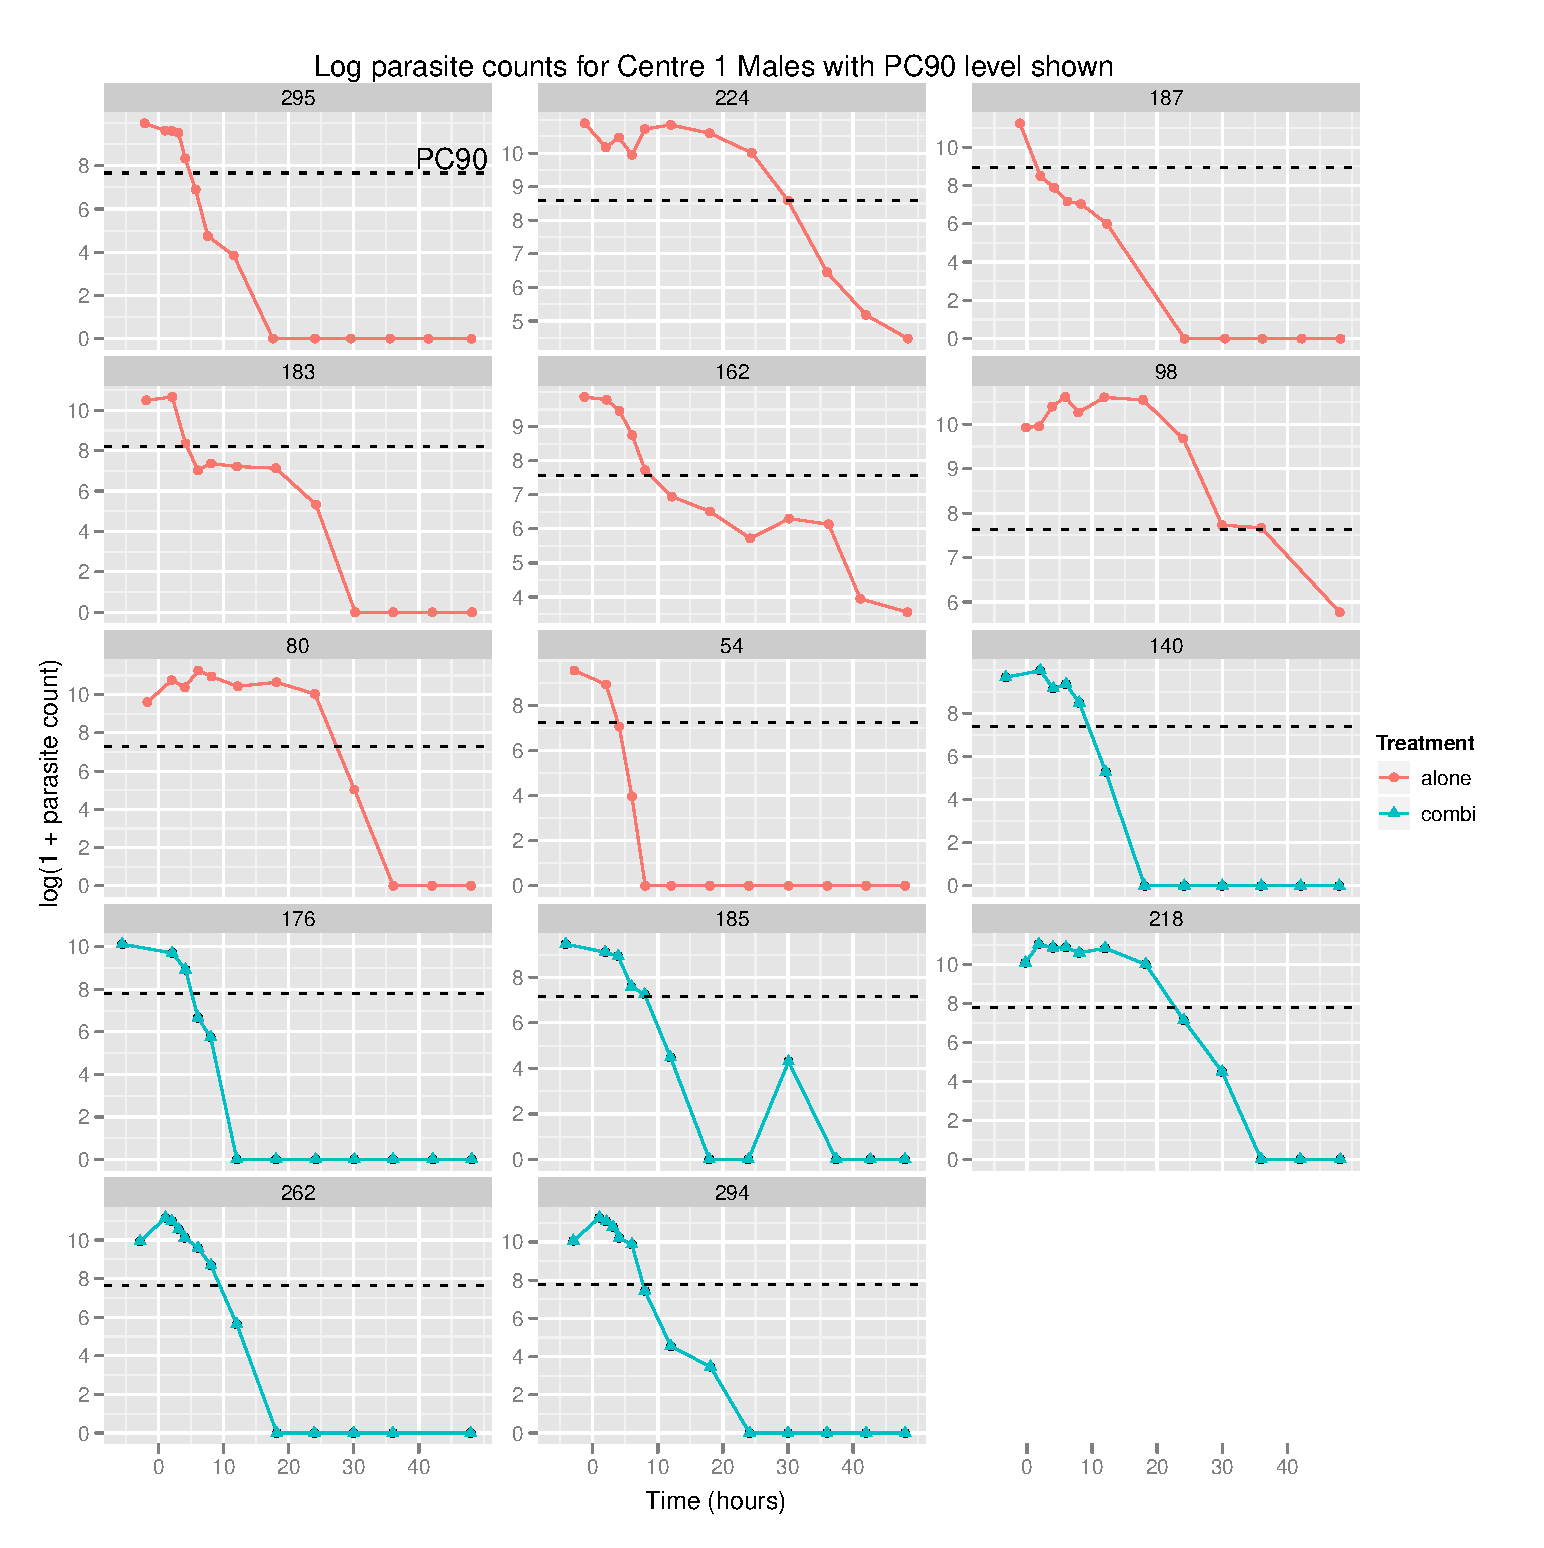
\includegraphics[width=6.1in]{log901M.eps}
\caption{Log parasite counts with PC90 level shown}
\label{log901M}
\end{center}
\end{figure}
\section{Regression modeling}
\subsection{Polynomial linear regression}
It was found that a cubic was the most suitable model, if we include the data only up to the first 0 parasite count. For some patients where the parasite count drops quickly to 0 a fit that includes the subsequent run of 0s would pull the cubic fit away from the most sensible estimate of PC90. It is more suitable for the purpose of estimating PC90 to only model the drop in the count to 0.

A cubic model was fitted to the log-transformed parasite count $P_{t}$ with time from first dose $t$ as the explanatory variable
$$\log(1+P_{t})=\beta_0+\beta_1t+\beta_2t^2+\beta_3t^3+\epsilon\quad\quad\epsilon\sim N(0,\sigma^2)$$

Figure \ref{cubics} shows the cubic fits to the log parasite count for centre 1, male subjects. It can be seen that the model describes the data fairly well, but it looks as if the combined treatment data is more closely modelled with the single treatment data showing more dispersion about the fitted model. 

The value of PC90 i.e. the time t at which the parasite count has fallen to 10\% was found by least-squares i.e. using the \texttt{optimize} function in R to minimise:
$$[log(1+0.1P_0)-\beta_0-\beta_1t-\beta_2t^2-\beta_3t^3]^2$$
where $P_0$ is the pre-treatment parasite count, $t$ is the time from first dose and $\beta_i$ are the fitted coefficients for the models for each of the 43 patients. Table \ref{pc90} shows the values of PC90 derived from the cubic fit to the parasite count by centre, sex and treatment.
\begin{figure}[h]
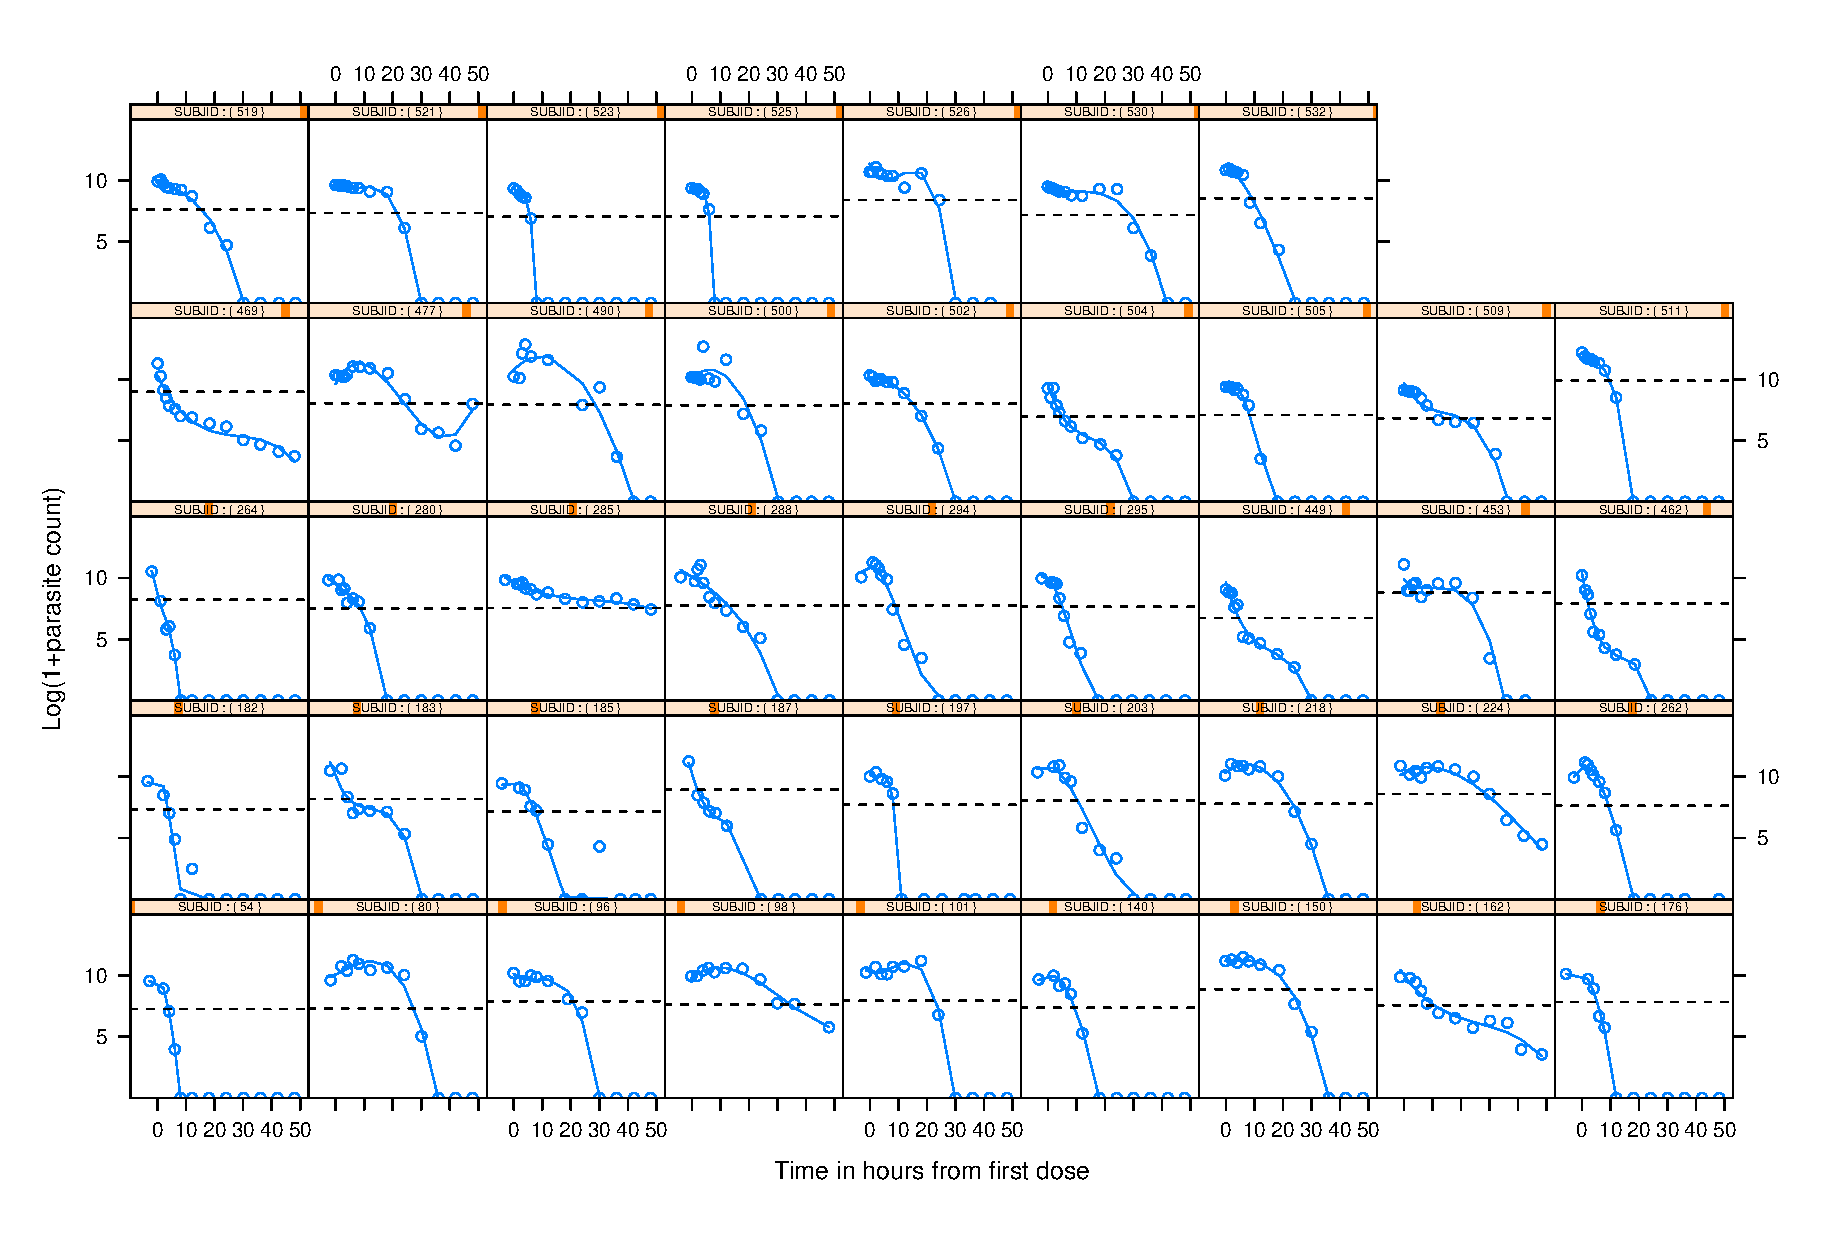
\includegraphics[width=6.1in]{cubics.eps} 
\caption{Cubic fits to log parasite count up to first zero reading}\label{cubics}
\end{figure}
\subsection{Non-linear logistic regression}
The logistic model fitted is
$$\log(1+P_t)=\alpha+\frac{\lambda}{1+e^{-\beta(t-\mu)}}+\epsilon$$
This was fitted to all the data as it can model a drop from an initial count level to a level of 0, unlike the cubic model. $\alpha$ is the lower asymptote which we would expect to be 0. $\alpha+\lambda$ is the upper asymptote which we would generally expect to be $P_0$ except in the cases where there is a marked increase in the parasite count after the first dose. $\beta$ determines the rate of reduction with time and $\mu$ is the point of inflection (maximum rate of reduction). This model was fitted using non-linear least-squares routines in \emph{R} and \emph{SAS}. Logistic fits to the same subjects as the cubic fits in Figure \ref{cubics} are shown in Figure \ref{logistics}.
\begin{figure}[h]
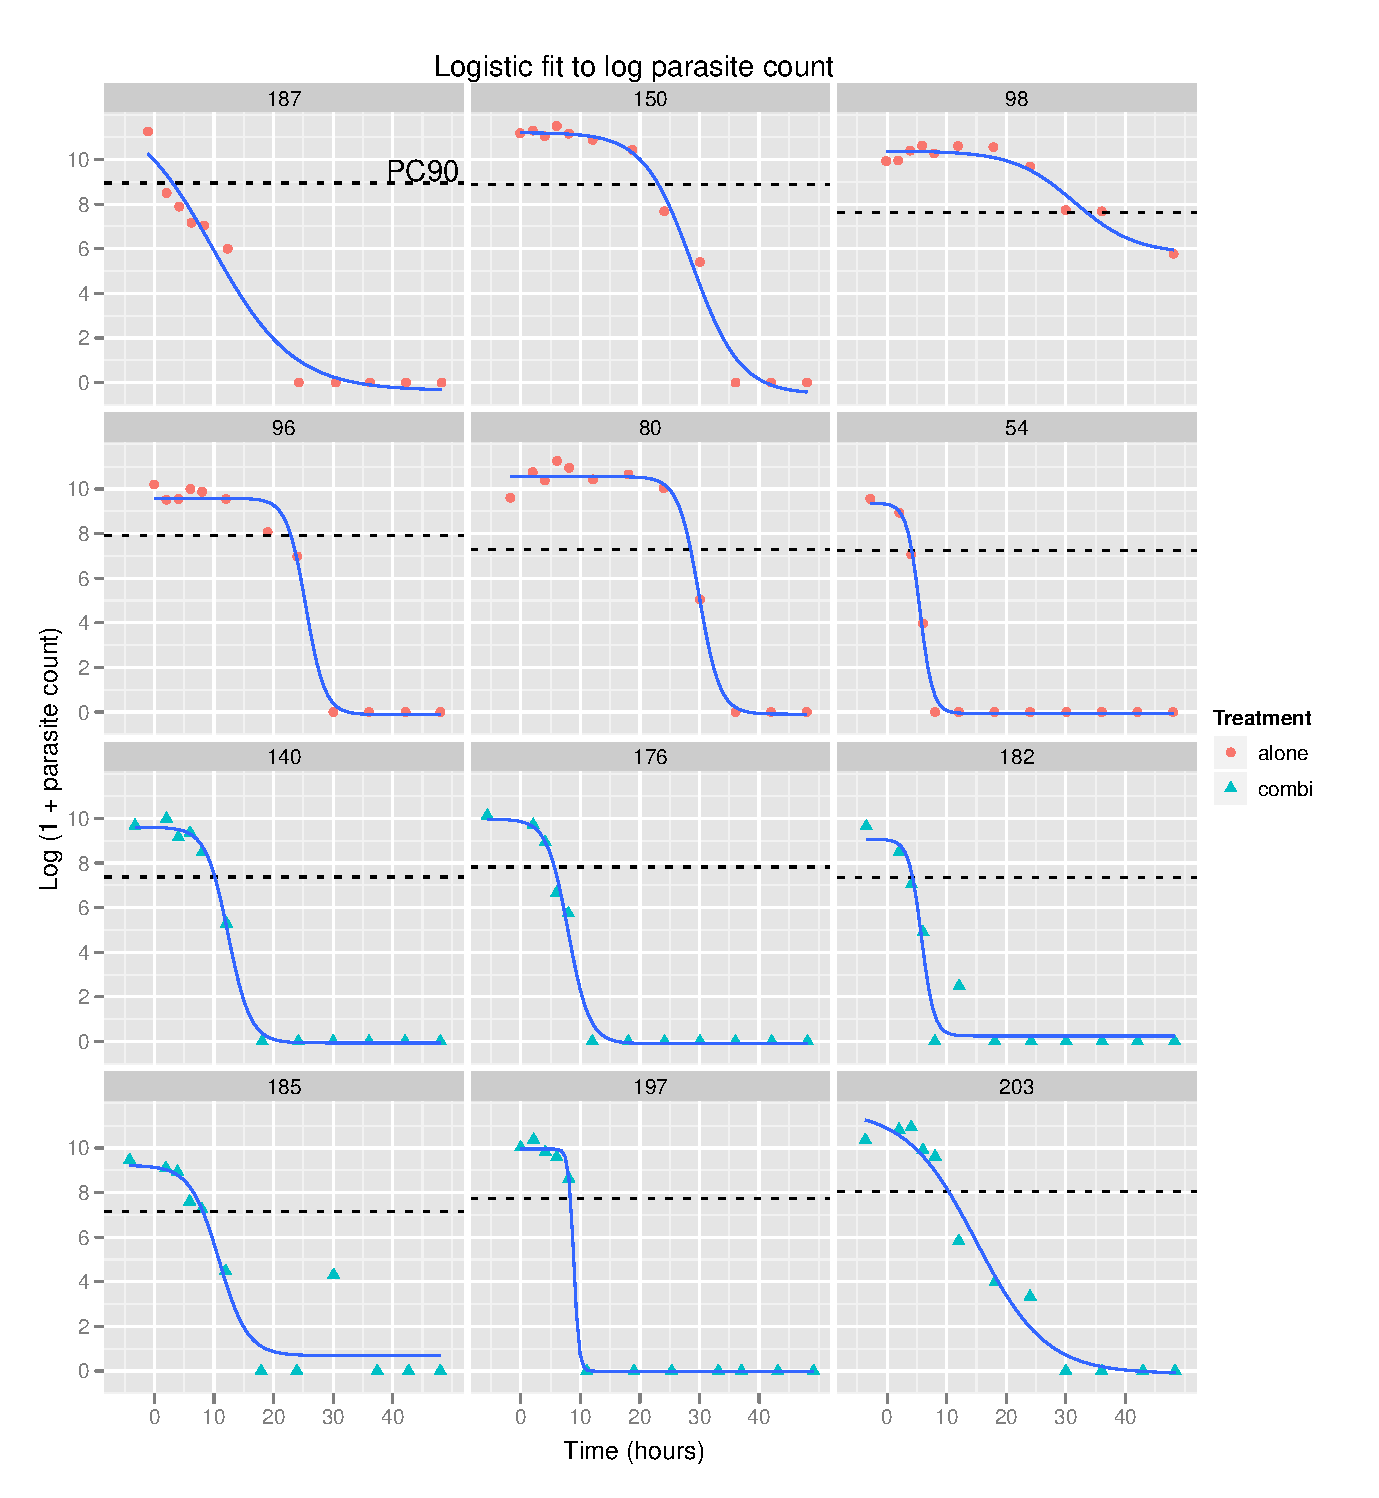
\includegraphics[width=6.1in]{logistics.eps} 
\caption{Logistic fits to log parasite count}\label{logistics}
\end{figure}
\subsubsection*{Choosing starting values for the parameters}
Figure \ref{logparms} shows the roles the parameters of the logistic model play in shaping the fitted curve. The non-linear, least-squares fitting routines (the \texttt{nls} function) in \emph{R} can take starting values for the parameters to be estimated. Looking at Figure \ref{logparms} it clearly follows that sensible starting values are:
\begin{itemize}
\item $\alpha$ = the minimum parasite count; usually 0.
\item $\lambda$ = the maximum minus the minimum count; usually the maximum.
\item $\mu$ = the time corresponding to the parasite count closest to halfway between the maximum and minimum counts.
\end{itemize} 
It was found by experimentation that the most suitable starting value for $\beta$ was -0.5, but that the fitting was insensitive to choice of $\beta$ if varied over the range of fitted $\beta$ values observed (and somewhat beyond).
\begin{figure}[h]
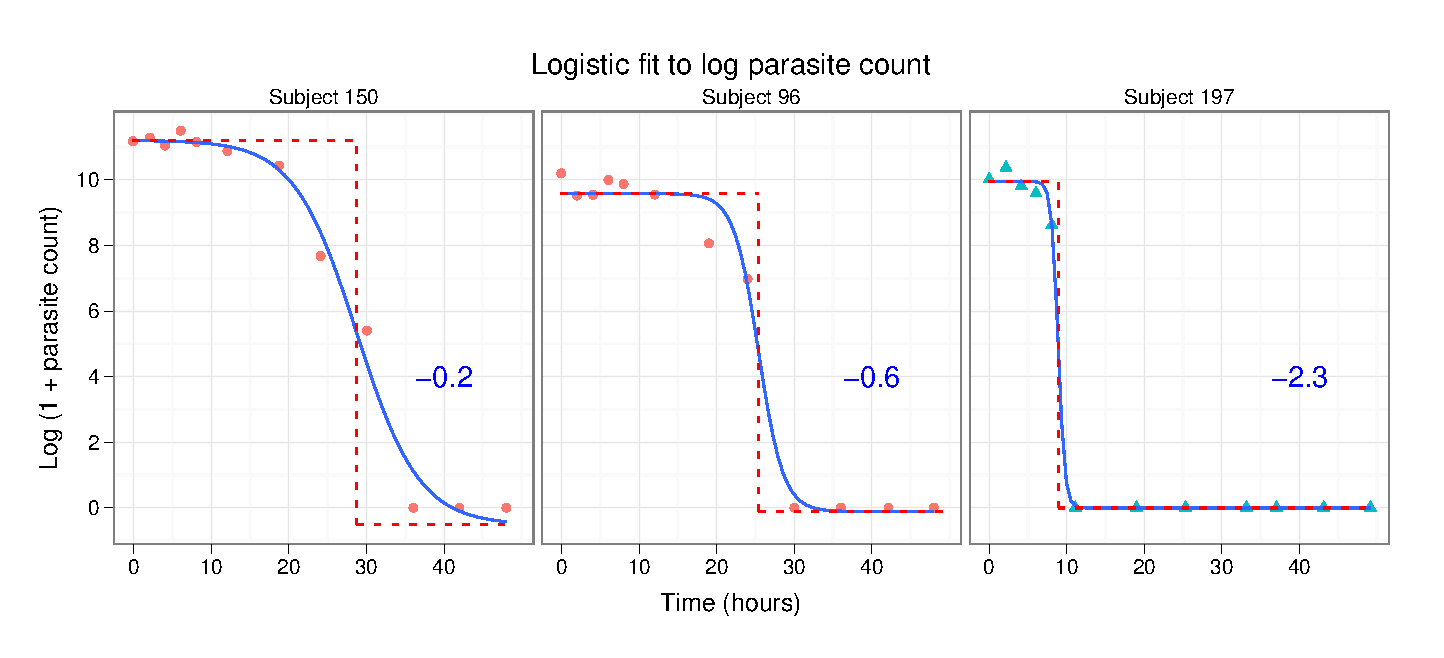
\includegraphics[width=6.1in]{logparms.eps} 
\caption{Illustration of parameters for logistic fits.\newline
The horizontal red lines show $\log(1+P_t)=\alpha$ (lower) and $\log(1+P_t)=\alpha+\lambda$ (upper), the vertical red line shows $t=\mu$ and the coefficient $\beta$ (rate of reduction) is given in blue.}\label{logparms}
\end{figure}

Despite careful selection of starting parameters, it was found that for several subjects that a logistic model is simply not appropriate. In these cases either the non-linear fitting routine failed to converge or, if convergence criteria were relaxed, would fit a model highly dependent on choice of starting parameters and when plotted with the data obviously does not model the data satisfactorily. The data for these subjects are shown in Figure \ref{failures}. 
\begin{figure}[h]
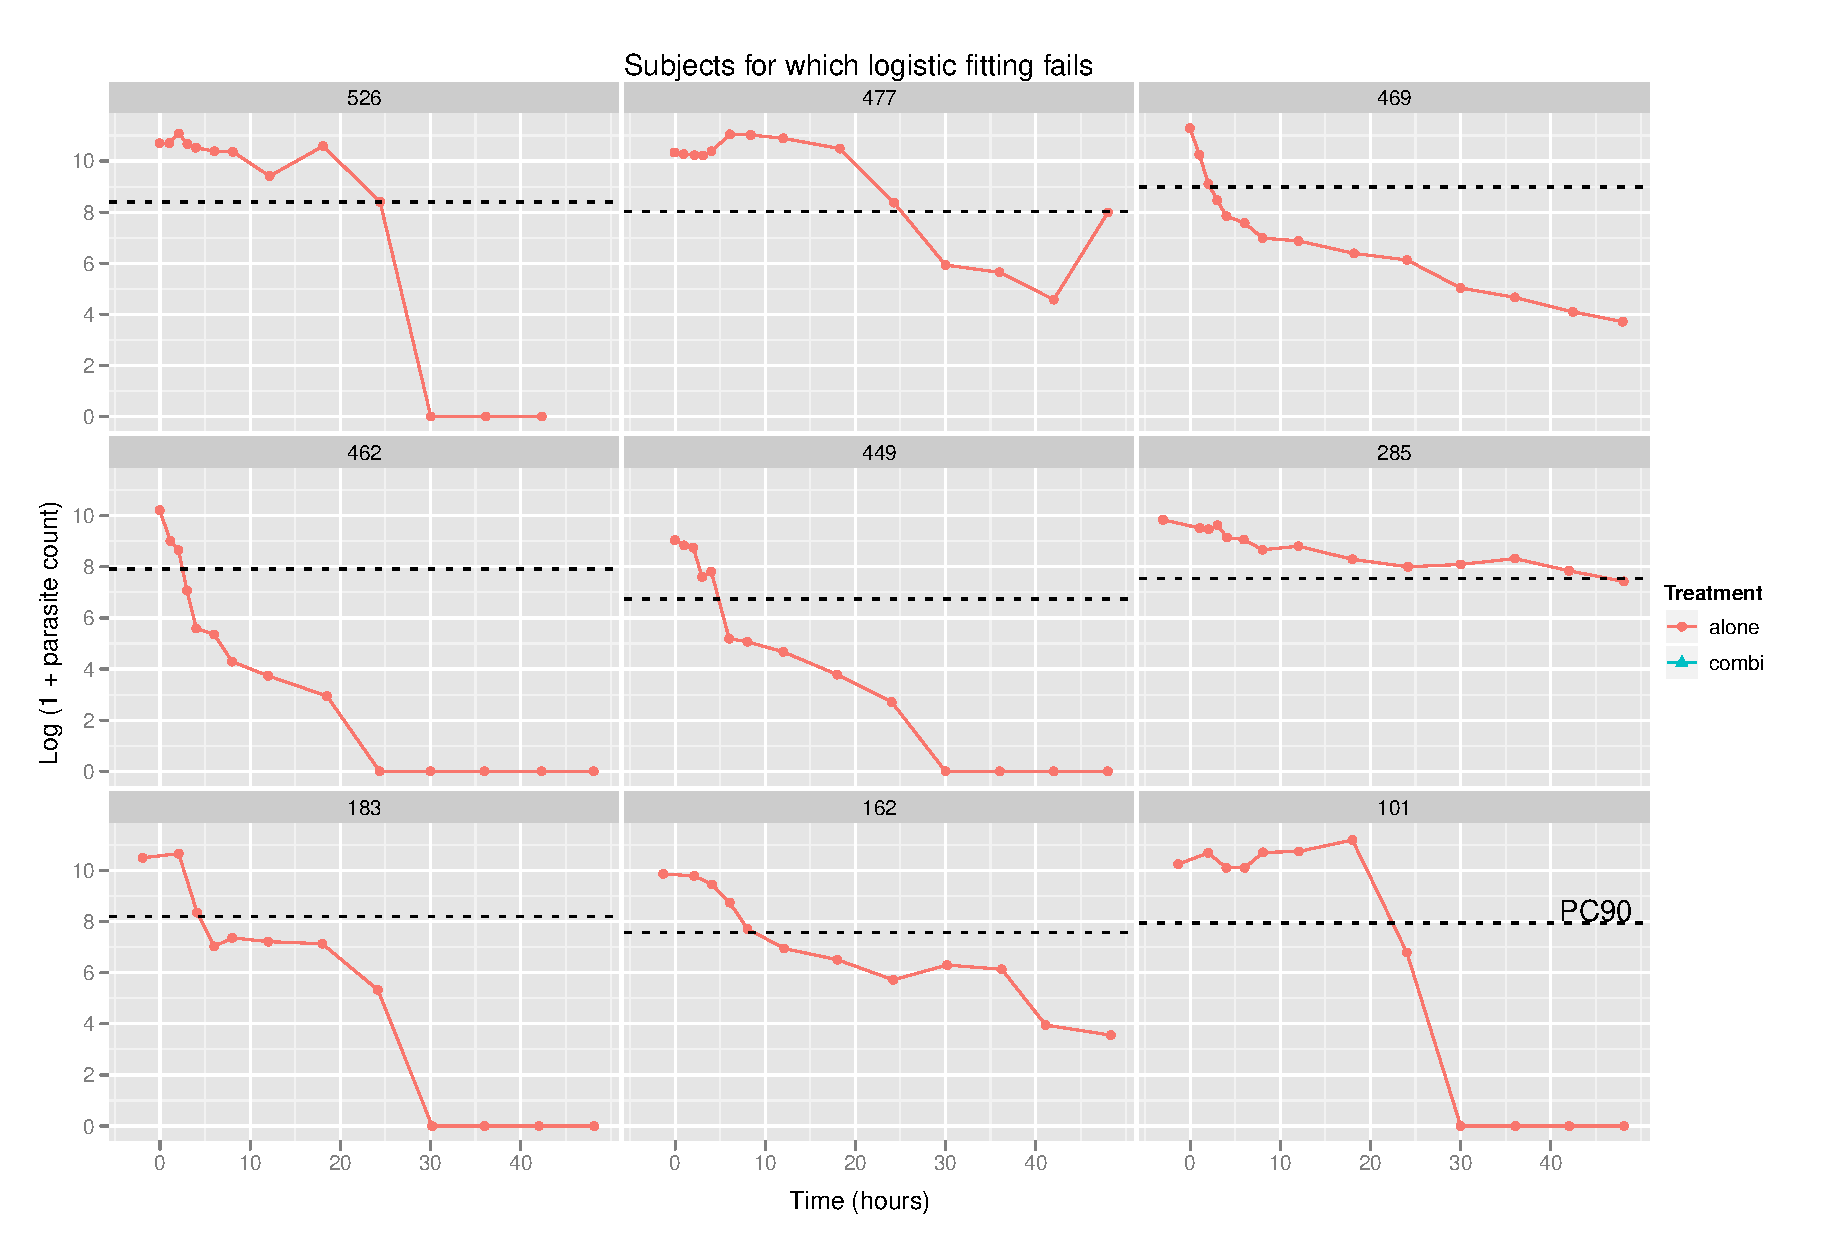
\includegraphics[height=4.2in]{failures.eps} 
\caption{Subjects for which the logistic fitting fails}\label{failures}
\end{figure}
\begin{figure}[h]
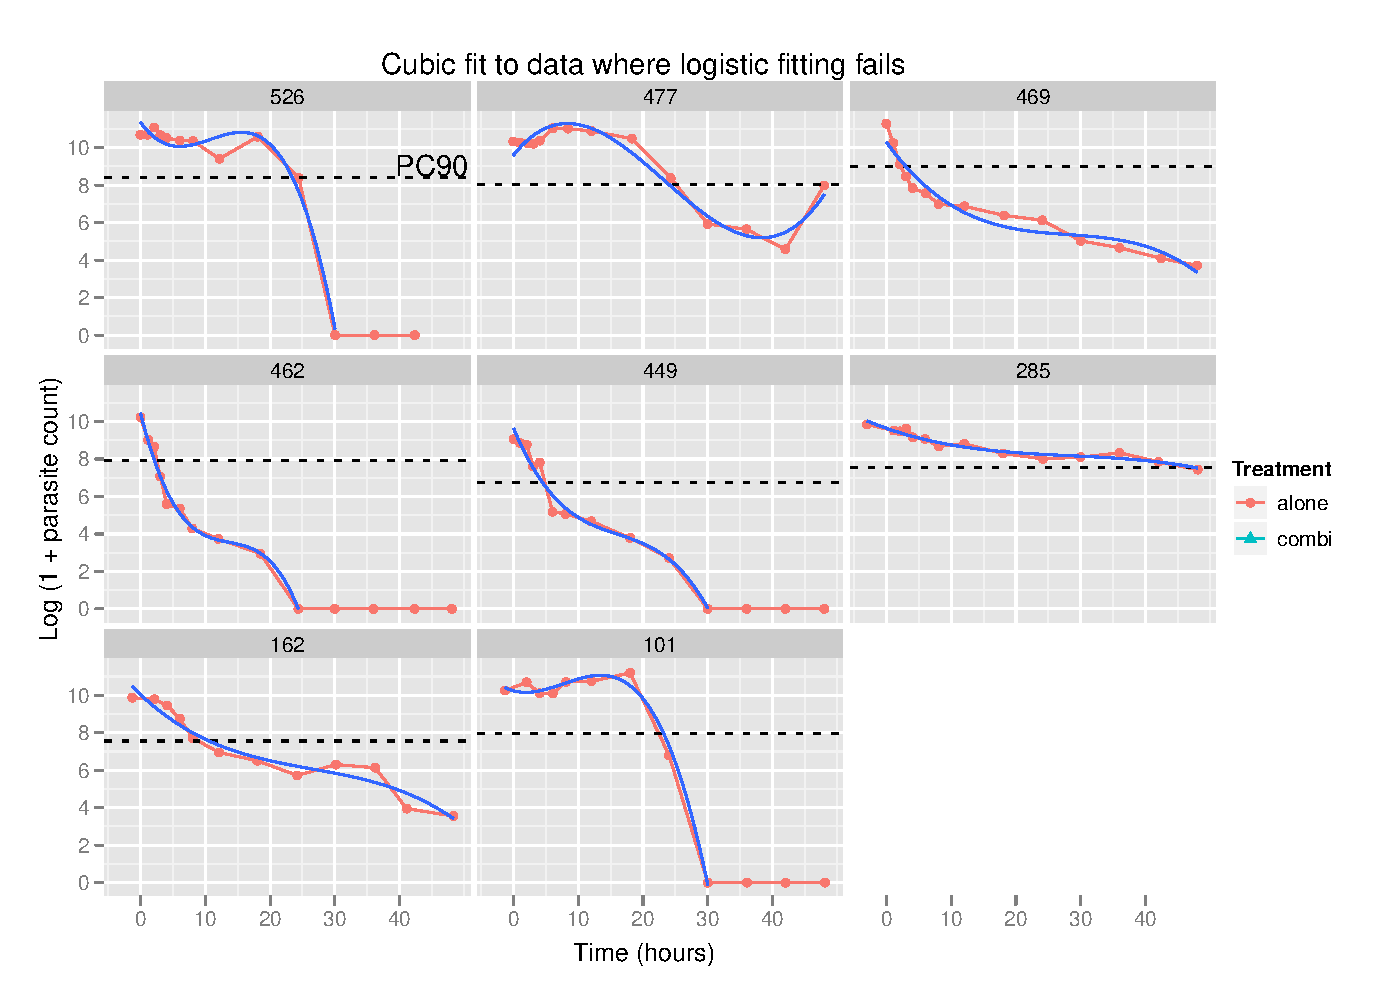
\includegraphics[height=4.2in]{failcubics.eps} 
\caption{Cubic fits to subjects where logistic fitting failed}\label{failcubics}
\end{figure}
\clearpage
\section{Interpolation}
The data points immediately above and below $0.1P_0$ were joined with a straight line fit and then the point where this line crosses $0.1P_0$ determines $t$ at PC90.

For loglinear interpolation the same procedure was performed only on a plot of $log(1+parct)$ vs. $t$.
\section{Comparison of results}
Figures \ref{1MB} and \ref{2FA} compare the logistic with the loglinear interpolation methods; the horizontal line is the PC90 level. It can be seen in Figure \ref{1MB} for Centre 1 male patients on treatment B that there is close agreement between the two methods. However in Figure \ref{2FA} for Centre 2 female patients on treatment A where the data is more ``erratic" that these simple approaches can fail in two ways.

Sometimes the non-linear fitting routine fails to converge on a solution (the plots with no logistic curve). This was found to be a problem using \texttt{nls} in \emph{R}. However, the \texttt{NLIN} routine in \emph{SAS} seems to achieve a reasonable solution in all cases. The second way in which this approach can fail is illustrated in the plot for patient 453 in Figure \ref{2FA} in that the parasite count temporarily dropped below the 10\% level before the actual final elimination of parasites had begun. It is clear that this approach should be modified to identify the \emph{last} time at which the parasite count drops below 10\%.

Table \ref{PC90} shows a comparison of the PC90 estimates by the four different methods looked at so far. Looking at the table the agreement in PC90 estimates looks fairly good. If we perform 6 paired-sample $t$-tests between pairs of methods we find that there is no strong evidence that the cubic regression and linear interpolation methods produce different estimates, likewise for the cubic and loglinear methods and the linear and logistic methods. The other combinations of methods do show evidence of difference in PC90 estimates ($P<0.0002$).

If we repeat the 3-way ANOVA of the previous report we find that \emph{Treatment} is the only factor that affects PC90 whichever method we use. Hence it would seem that the simplest method i.e. linear interpolation is the best method at this stage. However, as we know, the parasite count can be unreliable and depends on an operator-selected ``suitable" blood sample and so just one outlying value could throw the estimate by linear interpolation out as it only uses the two values above and below the PC90 count. In this respect an estimate based on more values should be more robust.
\begin{figure}
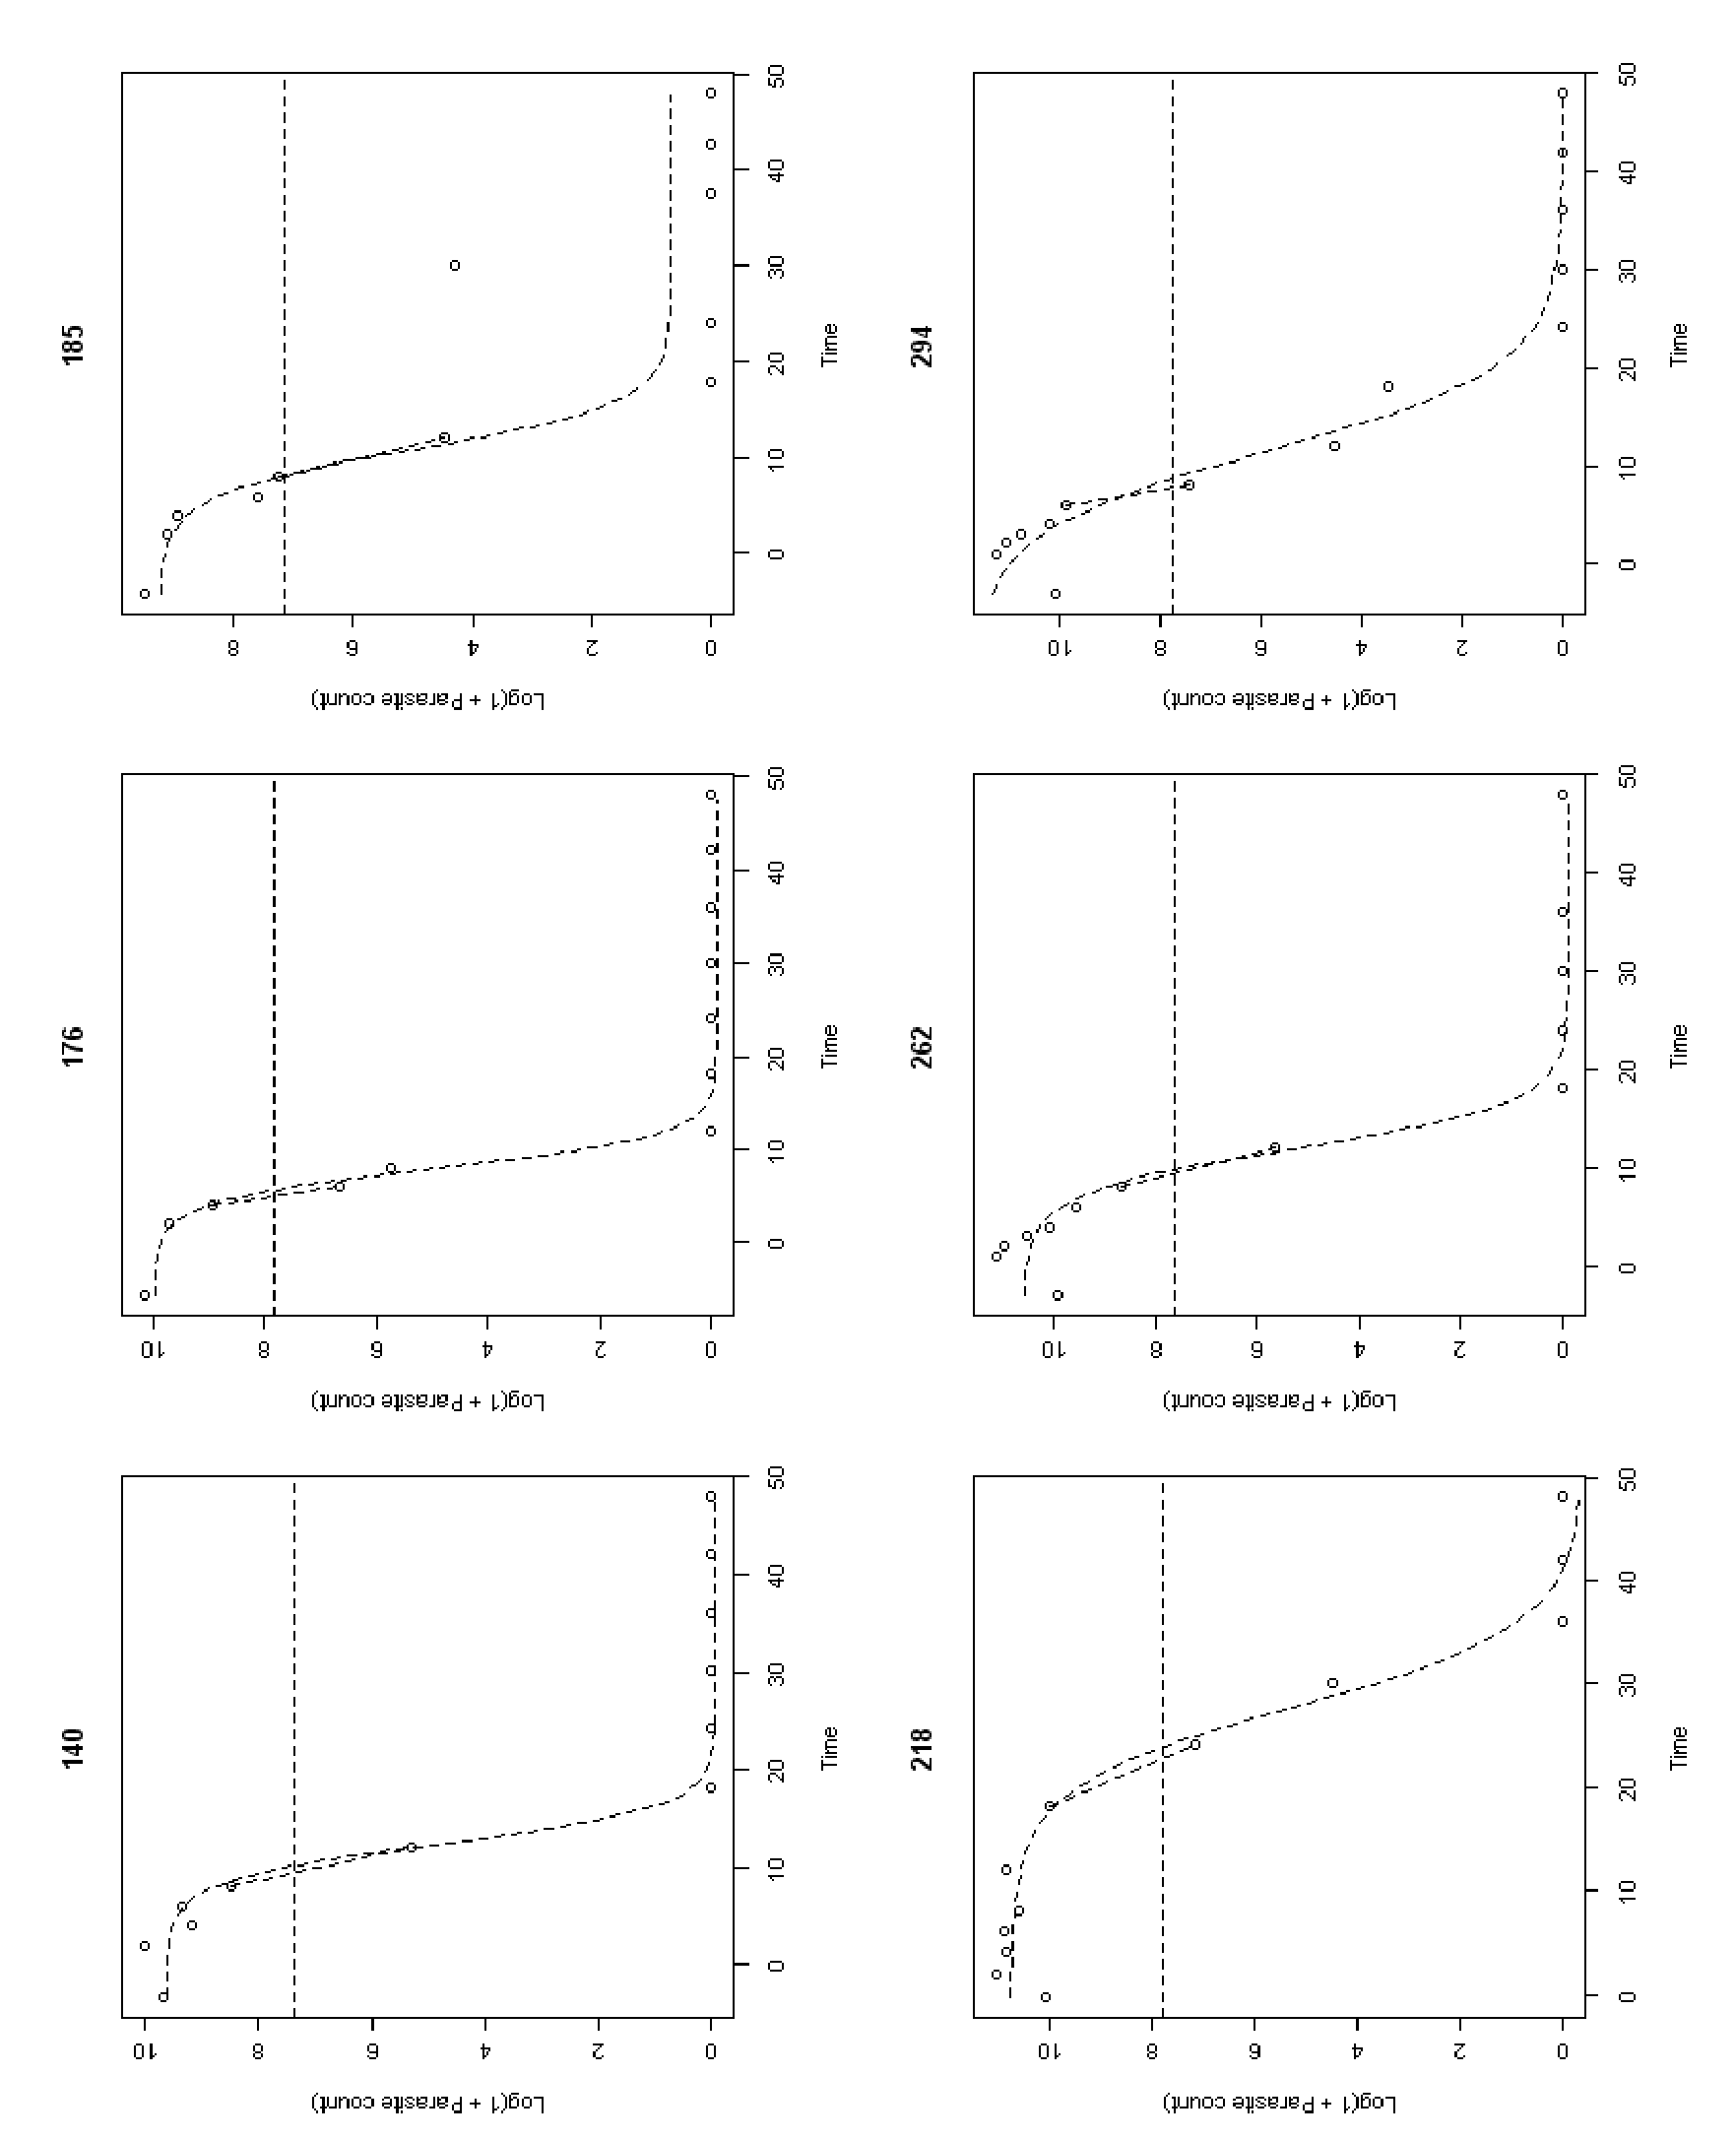
\includegraphics[scale=0.55]{logistic-1MB.eps} 
\caption{PC90 estimates for Centre 1 male patients on treatment B}\label{1MB}
\end{figure}
\begin{figure}
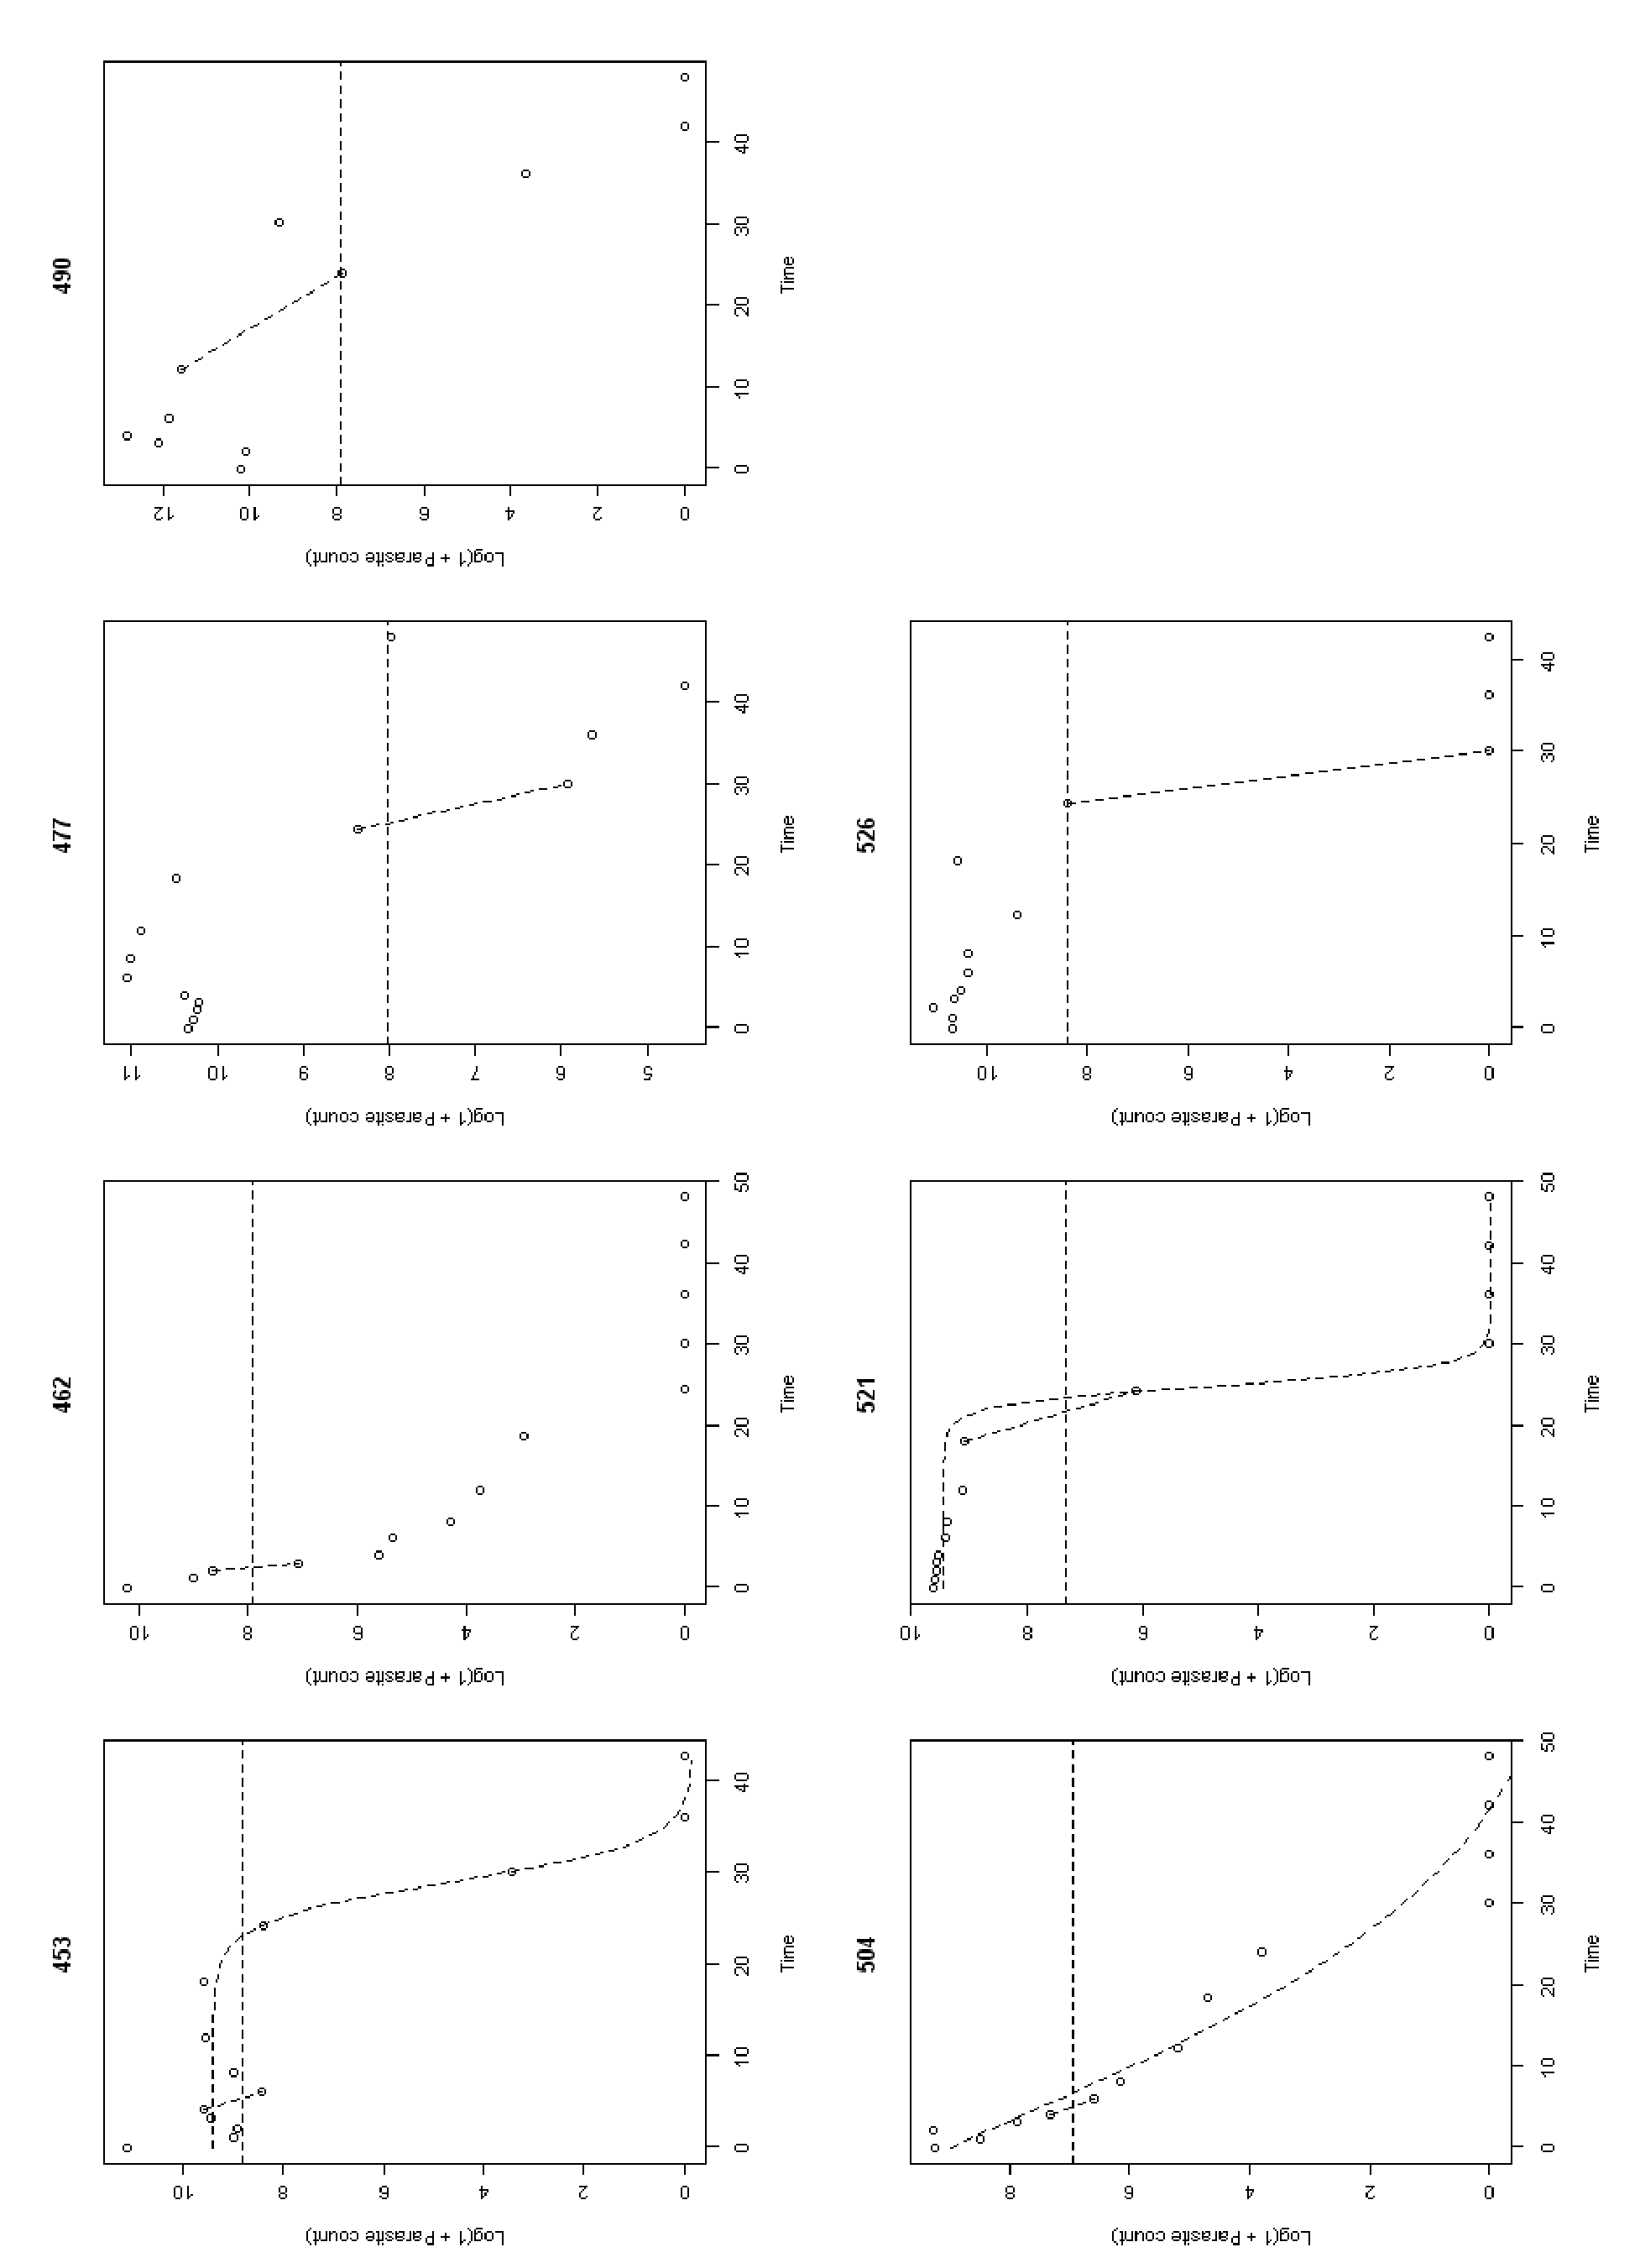
\includegraphics[scale=0.50]{logistic-2FA.eps} 
\caption{PC90 estimates for Centre 2 female patients on treatment A}\label{2FA}
\end{figure}
\begin{table}
\centering
\caption{Comparison of PC90 estimates by 4 methods}\label{PC90}
\begin{tabular}{|cccc|rrrr|}
\hline
Subject&Centre&&&PC90&PC90&PC90&PC90\\
ID&ID&Sex&Treatment&cubic&linear&loglinear&logistic\\
\hline
54&001&M&A&3.82&3.97&3.85&4.14\\
80&001&M&A&27.87&29.73&27.32&28.50\\
96&001&F&A&21.13&20.15&19.76&22.95\\
98&001&M&A&34.25&36.63&36.30&33.51\\
101&001&F&A&23.20&23.87&22.45&\\
140&001&M&B&9.49&10.90&9.46&10.16\\
150&001&F&A&22.53&23.24&21.75&23.12\\
162&001&M&A&9.79&9.10&8.84&\\
176&001&M&B&5.32&5.55&5.05&5.66\\
182&001&F&B&4.18&3.86&3.65&4.29\\
183&001&M&A&4.95&4.50&4.35&\\
185&001&M&B&7.70&8.33&8.09&8.13\\
187&001&M&A&0.83&1.93&1.53&3.05\\
197&001&F&B&8.64&9.87&8.15&8.35\\
203&001&F&B&9.44&11.27&9.69&10.30\\
218&001&M&B&23.54&23.76&22.77&23.92\\
224&001&M&A&28.86&30.02&30.01&30.26\\
262&001&M&B&9.40&10.74&9.40&9.85\\
264&001&F&B&0.88&0.96&0.85&1.43\\
280&001&F&B&8.61&9.92&9.04&9.72\\
285&001&F&A&47.24&46.76&46.52&\\
288&001&F&B&12.86&9.67&9.38&12.38\\
294&001&M&B&8.11&7.93&7.73&8.68\\
295&001&M&A&4.67&5.11&4.83&4.98\\
449&002&M&A&4.50&5.42&4.82&\\
453&002&F&A&20.07&22.73&21.97&23.08\\
462&002&F&A&2.22&2.67&2.49&\\
469&002&M&A&2.15&2.26&2.21&\\
477&002&F&A&24.03&26.10&25.08&\\
490&002&F&A&28.73&24.10&24.17&29.94\\
500&002&M&B&19.35&18.03&17.15&19.66\\
502&002&F&B&15.39&16.10&14.77&16.33\\
504&002&F&A&5.04&5.18&5.00&6.64\\
505&002&F&B&8.37&10.30&8.74&9.02\\
509&002&M&A&20.58&11.79&11.59&18.63\\
511&002&M&B&9.99&10.55&9.51&10.91\\
519&002&M&B&15.60&16.54&14.68&16.08\\
521&002&F&A&22.21&23.34&21.64&23.38\\
523&002&F&B&5.90&5.93&5.84&7.20\\
525&002&F&B&6.26&6.91&6.11&6.17\\
526&002&F&A&23.71&24.46&24.42&\\
530&002&M&A&29.07&29.53&28.09&29.28\\
532&002&M&B&8.94&8.33&8.08&9.21\\
\hline
\end{tabular}
\end{table}